\subsection{$d$-árna halda} 
\paragraph{Popis.}
Ako zovšeobecnenie binárnej haldy môžeme považovať d-árnu haldu. Rozdiel je v stupni vrcholov. 
%Každý vrchol v binárnej halde okrem listov má stupeň 2, v d-árnej halde je stupeň vrcholov $d$.
D-árna halda je, až na poslednú úroveň, \emph{úplný d-árny strom} spĺňajúci podmienku haldy. Posledná úroveň je 
\emph{zľava úplná}.
Halda sa najčastejšie reprezentuje v poli, koreň je na mieste $0$ a synovia $i$-teho prvku sú v poli na miestach 
$(d\cdot i + 1)$ až $(d\cdot i + d)$. V našej implementácií navyše každý vrchol obsahuje smerník na svojho otca a 
smerník na pole synov.
S takouto reprezentáciou v poli zľava úplný d-árny strom znamená, že v poli, v ktorom je uložený, nie sú "diery". 

\begin{figure}
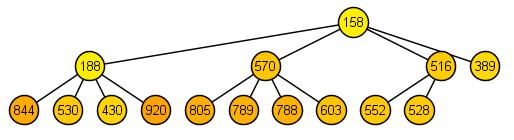
\includegraphics[width=\columnwidth]{obrazky/daryheap.png}
\caption{\emph{} 
Príklad d-árnej haldy pre $d = 4$} 
\label{img:komp} 
\end{figure}

\paragraph{Operácie.}
Operácia insert($x$) vloží vrchol s kľúčom $x$ na najbližšie voľné miesto, tak, aby sa neporušila úplnosť stromu 
a poslednej vrstvy. V praxi to znamená, že sa pridá nový prvok na koniec poľa. Takto vložený prvok môže porušovať 
podmienku haldy, takže ešte musí "prebublať" smerom hore na správne miesto. Vymieňa sa so svojím otcom, až pokým 
nie je podmienka haldy splnená.

Minimum sa nachádza v koreni haldy. Operácia \emph{deleteMin} najprv vymení koreň haldy s posledným vrcholom a potom 
minimum, ktoré sa teraz nachádza na konci haldy, odstráni. Koreň haldy po výmene nemusí spĺňať podmienku haldy a 
preto musí "prebublať" nadol. Vymieňa sa so svojím najmenším synom, až pokým nie je splnená podmienka.

Po zavolaní operácie decreaseKey($v, \Delta$) vrchol v nemusí spĺňať podmienku haldy a preto musí opäť 
"prebublať" nahor.

\paragraph{Časová zložitosť.}
Z popisu jednotlivých operácií sú zrejmé časové zložitosti. CreateHeap a findMin sa deje v konštantnom čase.
Ak n je počet prvkov v halde, potom operácie insert a decreaseKey majú časovú zložitosť $O(log_d(n))$, pretože 
$log_d(n)$ je hĺbka stromu, teda vrchol by sa po $log_d(n)$ krokoch dostal ku koreňu. Operácia deleteMin má 
zložitosť $O(d\cdot log_d(n))$, pretože sa navyše pri prebublávaní musí hľadať najmenší syn spomedzi $d$ synov.

\paragraph{Použitie.}
Z časových zložitostí platiacich pre binárnu haldu sa môže zdať vznik d-árnej haldy zbytočný. Avšak v mnohých 
reálnych prípadoch funguje zovšeobecnená verzia efektívnejšie. 
Jednak sú to príklady, keď operácie insert a decreaseKey sú využívané častejšie ako operácia deleteMin. Napríklad 
v Dijkstrovom algoritme pre najkratšie cesty v grafe funguje v určitých prípadoch d-árna halda rýchlejšie.
Navyše, pre niektoré konkrétne $d$ funguje d-árna halda rýchlejšie než binárna, vďaka tomu, že sa zníži počet 
prístupov na disk.

